\begin{frame}
	\frametitle{caso di studio: Karame [2012]}

	tipologia transazione
	\begin{itemize}
	  \item lenta, \textit{e.g.} acquisto ticket eventi
	  		\vspace{2pt}
	  		\newline sicurezza offerta dal mining
	  \vspace{5pt}
	  \item {\color{blue}veloce}, \textit{e.g.} pagamento in negozio
	  		\vspace{2pt}
	  		\newline $\exists$ possibilità di \textit{double spending}
	  		\begin{itemize}
	  			\item tempi scambio $[s]$ $\ll$ tempi validazione $[min]$
	  			\item Bitcoin segue tecnica \textit{struzzo}
	  			\item problema non grave ma aperto
	  		\end{itemize}
	\end{itemize}

\end{frame}
% ----------------------------------------------------------------------------------------------------------------------------
% \begin{frame}
% 	\frametitle{caso di studio: Karame [2012]}
% 	\framesubtitle{garantire validità nel caso \textit{veloce}}
% 	
% 	\begin{figure}[H]
% 	 	\begin{center}
% 			 \begin{tabular}{c @{\hspace{1em}} c}
% 				 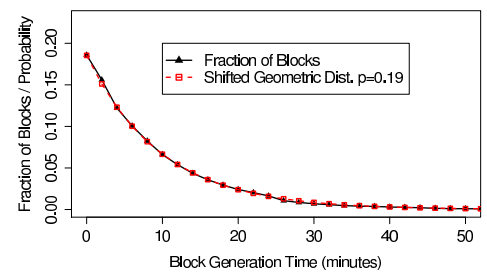
\includegraphics[height=5.5 cm]{images/dspending_1.png}
% 			 \end{tabular}
% 		 \end{center}
%  	\end{figure}
% 
% \end{frame}
% ----------------------------------------------------------------------------------------------------------------------------
\begin{frame}
	\frametitle{caso di studio: Karame [2012]}
	\framesubtitle{ipotesi}

	\begin{columns}
	 \begin{column}{.45\textwidth}
		hosts
		\begin{itemize}
		  \item $A$ peer disonesto
		  \item $H$ complici di $A$ 
		  \item $V$ vendor onesto
		\end{itemize}
		transazioni
		\begin{itemize}
		  \item $\orange{\mathfrak{T}_V}$: acquisto regolare
		  \item $\orange{\mathfrak{T}_A}$: recupero fraudolento
		\end{itemize}
	\end{column}
	
	\begin{column}{.65\textwidth}
		ipotesi
		\begin{itemize}
		  \item $A$ conosce indirizzo IP di $V$
		  \item $\mathcal{C}_A$ trascurabile
		  %SAY 
		  \item $\orange{\mathfrak{I}_V^{in}} = \orange{\mathfrak{I}_A^{in}} \in A$ 
		  \item $ V \ni\, \orange{\mathfrak{I}_V^{out}} \neq \orange{\mathfrak{I}_A^{out}} \in A$
		  \item implementazioni \textit{plain vanilla}
	 	\end{itemize}
 	\end{column}
 	\end{columns}

\end{frame}
% ----------------------------------------------------------------------------------------------------------------------------
\begin{frame}
	\frametitle{caso di studio: Karame [2012]}
	\framesubtitle{idea di massima}
 	
 	\begin{columns}
	 \begin{column}{.61\textwidth}
		\begin{itemize}	 
		  	\item $\orange{\mathfrak{T}_V}, \orange{\mathfrak{T}_A}$ inviate contemporaneamente
		  		\newline  $\;\;\Rightarrow $ incluse nello stesso pool
	  		\item se $\orange{\mathfrak{I}^{in}_\mathfrak{T}}=\orange{\mathfrak{I}^{in}_\mathfrak{T^\prime}}$ 
	  		%$\orange{\mathfrak{T}},\,\orange{\mathfrak{T^\prime}}$ condividono inputs 
	  			\newline $\;\;\Rightarrow $ non ammesse nello stesso pool
	  		\item inclusa solo la prima $\orange{\mathfrak{T}}$ ad arrivare
		  	$\;\;\;\;\;\;\;\;\Rightarrow$
		  	\begin{itemize}
		  		\item $\orange{\mathfrak{T}_A}$ da validare rapidamente
		  		\item $\orange{\mathfrak{T}_V}$ sarà smentita dalla rete
			\end{itemize}
		\end{itemize}
	 \end{column}
	
	 \begin{column}{.6\textwidth}
	 	\begin{figure}[H]
	 	\begin{center}
			 \begin{tabular}{c @{\hspace{1em}} c}
				 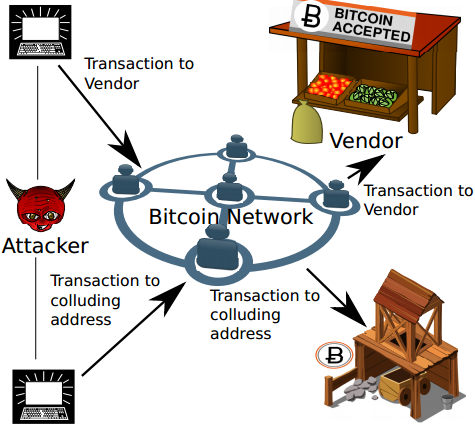
\includegraphics[height=5.5 cm]{images/dspending_2.png}
			 \end{tabular}
		 \end{center}
 		\end{figure}
	 \end{column}
	\end{columns}

\end{frame}
% ----------------------------------------------------------------------------------------------------------------------------
\begin{frame}
	\frametitle{caso di studio: Karame [2012]}
	\framesubtitle{$\mathbf{1^a}$ \textbf{condizione}: connessione diretta tra $A$ e $V$}
	
	\fbox{$V$\,riceve prima\,$\orange{\mathfrak{T}_V}$\,di\,$\orange{\mathfrak{T}_A}$}
	\newline oppure\,$V$\,includerebbe prima\,$\orange{\mathfrak{T}_A}$\,nel suo pool
	
	\begin{columns}
		\begin{column}{.5\textwidth}
			\begin{itemize}
			  \item client accetta sempre nuove connessioni < 125 max
			  \item $A$ comunica con $H$
				\begin{itemize}
					\item senza latenza
					\item privatamente    
				\end{itemize}
			  \item $H$ non comunica con $V$
			  \item $A$ invia
				\begin{enumerate}
				  \item $\orange{\mathfrak{T}_V}$ a $V$
				  \item $\orange{\mathfrak{T}_A}$ a $H$
				\end{enumerate}
			\end{itemize}
			 $\;\;\;\;$\fbox{$\Rightarrow \orange{t_V^V} < \orange{t_V^A}$}
		\end{column}
		
		\begin{column}{.60\textwidth}
			\begin{figure}[H]
		 	\begin{center}
				 \begin{tabular}{c @{\hspace{1em}} c}
					 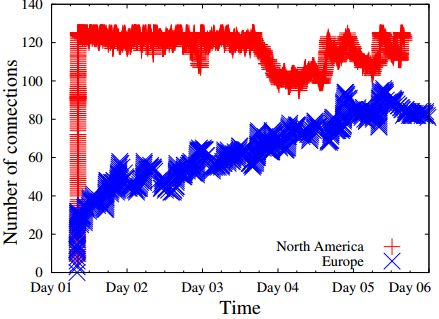
\includegraphics[height=4.75 cm]{images/dspending_3.png}
				 \end{tabular}
			 \end{center}
				\caption{analisi del momento propizio}
	 		\end{figure}
		\end{column}
	\end{columns}		  
\end{frame}
% ----------------------------------------------------------------------------------------------------------------------------
\begin{frame}
	\frametitle{caso di studio: Karame [2012]}
	\framesubtitle{$\mathbf{2^a}$ \textbf{condizione}: diffusione manipolata}
	
	\fbox{$\orange{\mathfrak{T}_A}$ confermata in \textit{blockchain} prima di $\orange{\mathfrak{T}_V}$} 
	\newline oppure $\orange{\mathfrak{T}_A}$ non più validabile
	  		
	\begin{itemize}
	  \item $\text{ogni peer include}\;\orange{\mathfrak{T}_A}\:\dot{\vee}\:\orange{\mathfrak{T}_V}\;\text{in proprio pool}$
	  \begin{itemize}
	  	\item $\orange{\mathfrak{T}_A}, \orange{\mathfrak{T}_V}$ broadcastate in due partizioni 
		\item termine quando $\orange{\mathfrak{T}_A}\:\dot{\vee}\:\orange{\mathfrak{T}_V}$ confermata
 	  \end{itemize}
	  \item \fbox{$\Pr[\orange{\tau_A} < \orange{\tau_V}] \propto \sfrac{\orange{\eta_A}}{\orange{\eta_V}}$} migliora se
		\begin{itemize}
			\item invio di $\orange{\mathfrak{T}_A}$ precede invio di $\orange{\mathfrak{T}_V}$ 
			\item $H$ aiutano $A$ diffondendo $\orange{\mathfrak{T}_A}$ e filtrando $\orange{\mathfrak{T}_V}$ 
		\end{itemize}
% 	  \item ulteriori ipotesi
% 	  	\begin{itemize}
% 	  	  	\item $\exists$ istante ove $\orange{\mathfrak{T}_A},\,\orange{\mathfrak{T}_V}$ convivono
% 	  	  	\item $\forall\,\orange{\varepsilon}\;\mathrm{p.a.p.},\;\;\;
% 	  	  			\Pr[\orange{\tau_A}\sim\mathrm{secs}]\cup\Pr[\orange{\tau_V}\sim\mathrm{secs}]<\orange{\varepsilon}$ 
%   			\item $\orange{\eta_A},\,\orange{\eta_V}$ non scambiano blocchi risolti $\Rightarrow \orange{\tau_A},\,\orange{\tau_V}$ indipendenti
% 	  	\end{itemize}
	\end{itemize}

\end{frame}
% ----------------------------------------------------------------------------------------------------------------------------
\begin{frame}
	\frametitle{caso di studio: Karame [2012]}
	\framesubtitle{probabilità di successo}

	$\Pr[\text{successo in tempo}\;\orange{\delta t}] \sim \mathrm{Bernoulli}(\orange{\eta_A},\,\orange{p})$
	\begin{itemize}
	  \item $\orange{\eta_A}=$ \# peers coinvolti
	  \item $\orange{p}=\Pr[\,\text{peer generi}\:\orange{\mathfrak{B}}\:\text{in}\;{\orange{\delta t}}\,]$ 
	\end{itemize}

	\begin{figure}[H]
	 	\begin{center}
			 \begin{tabular}{c @{\hspace{1em}} c}
				 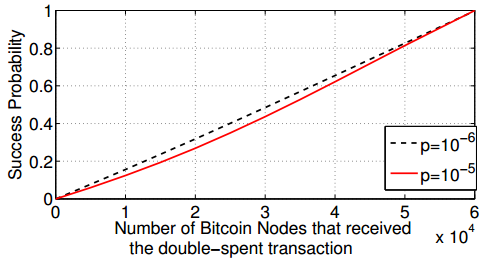
\includegraphics[height=4.5 cm]{images/dspending_4.png}
			 \end{tabular}
		 \end{center}
		 \caption{$\Pr[\mathrm{successo}\;|\;\delta t=\orange{10s},\;\eta=\orange{6\cdot10^4}]$}
 	\end{figure}
 	
\end{frame}